\newpage

\section{Badanie ankietowe wśród pracowników branży IT}
By móc udzielić trafniejszej odpowiedzi na pytanie postawione w tytule pracy, analiza literatury została dodatkowo wsparta badaniem ankietowym przeprowadzonym wśród pracowników branży informatycznej.

\subsection{Cel badania}
Celem badania było zidentyfikowanie kluczowych kompetencji, które powinien posiadać skuteczny kierownik projektu informatycznego na podstawie dotychczasowych doświadczeń pracowników branży informatycznej. Dodatkowym aspektem tego badania w porównaniu do innych dostępnych prac było szczególne zwrócenie uwagi na umiejętności z zakresu inżynierii oprogramowania. Co pozwoliło na bardziej dokładne określienie wartości poszczególnych kompetencji technicznych i na jakim poziomie powinny być one posiadane przez kierownika projektu informatycznego. Poruszona została również kwestia szans i zagrożeń wynikających z posiadania przez kierownika projektu wiedzy technicznej.

\subsection{Metodologia oraz opis badania}
Badanie zostało przeprowadzone w formie dorbowolnej i anonimowej ankiety internetowej. Dostęp do ankiety był ograniczony, każdy z respondentów był indywidualnie zapraszany do udziału w badaniu. W badaniu wzięli udział pracownicy różnych przedsiębiorstw i poziomów organizacyjnych, co pozwoliło na uzyskanie szerokiego obrazu. 

Ankieta została podzielona na trzy sekcje. Pierwsza część dotyczyła ogólnych informacji o respondentach, takich jak ich doświadczenie zawodowe, stanowisko oraz rodzaj projektów, w których uczestniczyli. Druga część skupiła się na ocenie kompetencji kierownika projektu w różnych obszarach, takich jak umiejętności interpersonalne, przywódcze, techniczne i analityczne. W tej części ankietowani wartościowali znaczenia różnych kompetencji kierownika projektu w skali Likerta (1–5), gdzie 1 oznacza brak znaczenia, a 5 oznacza bardzo wysokie znaczenie. Ostatnia część ankiety skupiona była na aspekcie umiejętności z zakresu inżynierii oprogramowania. Oprócz pytań zamkniętych bezpośrednio nawiązujących do pytania zadanego w tytule pracy, respondenci mieli możliwość na bardziej szczegółowe wyrażenie opinii w formie pytań otwartych.
Ankieta została skonstruowana w taki sposób, aby umożliwić respondentom ocenę zarówno kompetencji technicznych, jak i miękkich. W szczególności zwrócono uwagę na umiejętności związane z inżynierią oprogramowania, które są kluczowe w kontekście zarządzania projektami informatycznymi.
Badanie zostało zrealizowane w formie anonimowej ankiety internetowej. Wzięło w nim udział 30 respondentów reprezentujących różne stanowiska w sektorze IT. Kwestionariusz zawierał pytania zamknięte , a także pytania otwarte, umożliwiające rozszerzenie odpowiedzi o opinie jakościowe.

\subsection{Charakterystyka próby}

Wśród respondentów dominowali programiści (20 osób), następnie kierownicy projektów (5 osób) oraz inne role (5 osób). Większość ankietowanych jest pracownikami branży informatycznej ponad 5 lat, dzięki czemu ich odpwiedzi są wspartę dużą wiedzą empiryczną. Dodatkowo w badaniu wzięli udział pracownicy mający doświadczenie w różnych typach projektów, co pozwoliło na uzyskanie szerokiego obrazu sytuacji. Co trzeci ankietowany miał również doświadczenie na stanowisku kierowniczym.

\begin{figure}
  \caption{Czas pracy w branży IT}
  \centering
  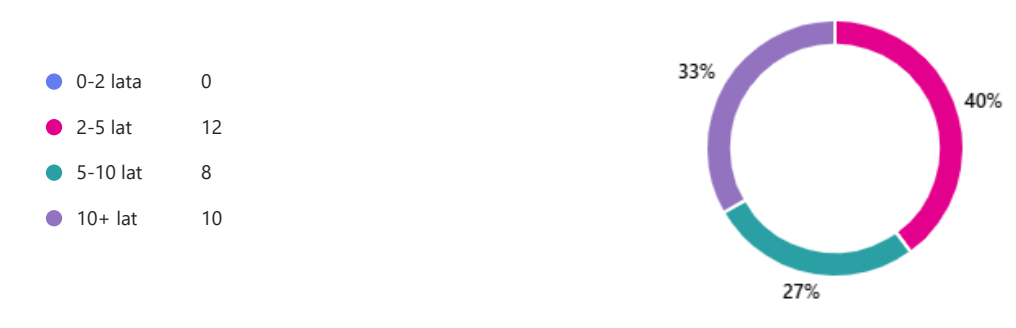
\includegraphics[width=1\linewidth]{doswiadczenie.PNG}
  \caption*{Źródło: Badanie własne}
\end{figure}

\begin{figure}
  \caption{Charakter realizowanych projektów}
  \centering
  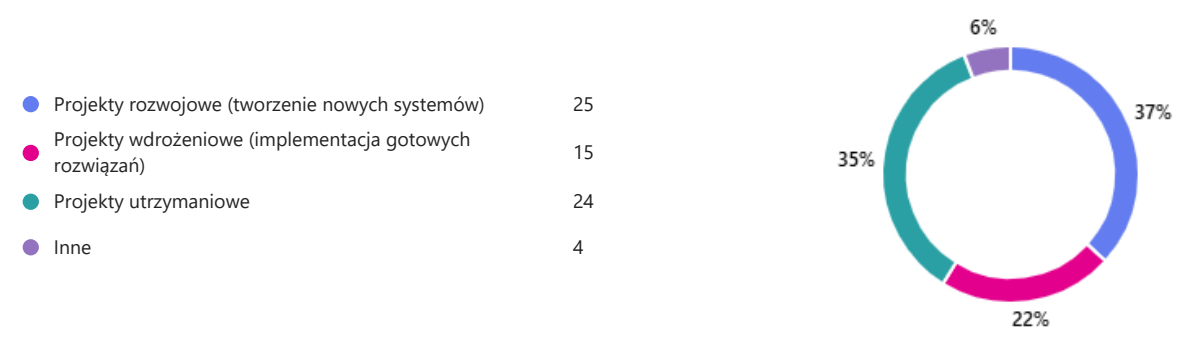
\includegraphics[width=1\linewidth]{projekty.png}
  \caption*{Źródło: Badanie własne}
\end{figure}

\subsection{Wyniki badania}

\subsubsection{Wyniki badania}

\begin{longtable}{p{10cm} r}
  \caption{Średnie oceny kompetencji kierownika projektu IT}
  \toprule
  \textbf{Kategoria} & \textbf{Średnia} \\
  \midrule
  \multicolumn{2}{l}{\textbf{Kompetencje interpersonalne i komunikacyjne}} \\
  Umiejętności komunikacyjne & 4{,}67 \\
  Empatia i umiejętność słuchania & 4{,}23 \\
  Negocjacje i rozwiązywanie konfliktów & 4{,}17 \\
  \textbf{Średnia kategorii} & \textbf{4{,}36} \\
  \midrule
  \multicolumn{2}{l}{\textbf{Kompetencje przywódcze i zarządcze}} \\
  Przywództwo i motywowanie & 3{,}97 \\
  Zarządzanie zespołem i delegowanie & 4{,}23 \\
  Zarządzanie czasem i organizacja pracy & 4{,}43 \\
  \textbf{Średnia kategorii} & \textbf{4{,}21} \\
  \midrule
  \multicolumn{2}{l}{\textbf{Kompetencje strategiczne i analityczne}} \\
  Myślenie strategiczne & 4{,}17 \\
  Zarządzanie ryzykiem & 4{,}17 \\
  Zdolność do podejmowania decyzji & 4{,}4 \\
  Znajomość i rozumienie domeny biznesowej & 4{,}07 \\
  \textbf{Średnia kategorii} & \textbf{4{,}21} \\
  \midrule
  \multicolumn{2}{l}{\textbf{Kompetencje finansowe i organizacyjne}} \\
  Zarządzanie budżetem i zasobami & 3{,}6 \\
  Orientacja na wyniki i efektywność & 3{,}77 \\
  Wiedza teoretyczna z zakresu zarządzania projektami & 3{,}1 \\
  \textbf{Średnia kategorii} & \textbf{3{,}49} \\
  \midrule
  \multicolumn{2}{l}{\textbf{Kompetencje personalne}} \\
  Odporność na stres & 3{,}83 \\
  Cierpliwość & 3{,}9 \\
  Chęć rozwoju i uczenia się & 3{,}3 \\
  \textbf{Średnia kategorii} & \textbf{3{,}68} \\
  \midrule
  \multicolumn{2}{l}{\textbf{Kompetencje z zakresu inżynierii oprogramowania}} \\
  Formułowanie wymagań dotyczących oprogramowania & 3{,}57 \\
  Metody testowania i weryfikacji poprawności & 2{,}73 \\
  Cykl życia systemów informatycznych & 2{,}5 \\
  Znajomość wzorców projektowych i architektonicznych & 2{,}15 \\
  Umiejętność programowania & 2{,}17 \\
  Wiedza w zakresie baz danych & 2{,}27 \\
  Wiedza w zakresie algorytmów i struktur danych & 1{,}93 \\
  Znajomość systemów operacyjnych, sieci komputerowych i bezpieczeństwa & 2{,}17 \\
  \textbf{Średnia kategorii} & \textbf{2{,}67} \\
  \bottomrule
  \caption*{Źródło: Badanie własne}
  \end{longtable}

\subsubsection*{4.1 Porównanie średnich ocen kompetencji}

Na podstawie powyższych danych najwyżej oceniono kompetencje interpersonalne i komunikacyjne, co potwierdza ich fundamentalne znaczenie w roli kierownika projektu IT.



\subsubsection*{4.2 Analiza szczegółowa}

W obszarze kompetencji interpersonalnych najwyżej oceniono umiejętność komunikowania się z zespołem, a także empatię i zdolność rozwiązywania konfliktów. W kompetencjach przywódczych dominowały takie cechy jak zdolność motywowania, delegowania oraz zarządzanie czasem.

Kompetencje strategiczne obejmowały myślenie analityczne, podejmowanie decyzji i zarządzanie ryzykiem — wszystkie uzyskały wysokie noty. Kompetencje techniczne, mimo niższych ocen ogólnych, zostały uznane za istotne w kontekście określonych ról projektowych.

\subsection*{5. Wyniki jakościowe}

Respondenci wskazali, że brak wiedzy technicznej u kierownika może prowadzić do:

\begin{itemize}
  \item opóźnień harmonogramowych,
  \item trudności w koordynacji zadań,
  \item nieporozumień między zespołem a kierownikiem.
\end{itemize}

Jednocześnie, nadmierne skupienie na aspektach technicznych może skutkować:

\begin{itemize}
  \item mikrozarządzaniem,
  \item brakiem perspektywy biznesowej,
  \item paraliżem decyzyjnym.
\end{itemize}

\subsection*{6. Wnioski}

Badanie potwierdziło hipotezy sformułowane na podstawie literatury — kompetencje społeczne (interpersonalne i przywódcze) mają kluczowe znaczenie dla skutecznego zarządzania projektami IT. Jednocześnie nie można ignorować roli wiedzy technicznej, która w odpowiednich proporcjach wspiera procesy zarządcze, komunikację z zespołem oraz rozumienie ryzyka projektowego.

\printbibliography

\end{document}

